% Options for packages loaded elsewhere
\PassOptionsToPackage{unicode}{hyperref}
\PassOptionsToPackage{hyphens}{url}
%
\documentclass[
]{article}
\usepackage{amsmath,amssymb}
\usepackage{lmodern}
\usepackage{iftex}
\ifPDFTeX
  \usepackage[T1]{fontenc}
  \usepackage[utf8]{inputenc}
  \usepackage{textcomp} % provide euro and other symbols
\else % if luatex or xetex
  \usepackage{unicode-math}
  \defaultfontfeatures{Scale=MatchLowercase}
  \defaultfontfeatures[\rmfamily]{Ligatures=TeX,Scale=1}
\fi
% Use upquote if available, for straight quotes in verbatim environments
\IfFileExists{upquote.sty}{\usepackage{upquote}}{}
\IfFileExists{microtype.sty}{% use microtype if available
  \usepackage[]{microtype}
  \UseMicrotypeSet[protrusion]{basicmath} % disable protrusion for tt fonts
}{}
\makeatletter
\@ifundefined{KOMAClassName}{% if non-KOMA class
  \IfFileExists{parskip.sty}{%
    \usepackage{parskip}
  }{% else
    \setlength{\parindent}{0pt}
    \setlength{\parskip}{6pt plus 2pt minus 1pt}}
}{% if KOMA class
  \KOMAoptions{parskip=half}}
\makeatother
\usepackage{xcolor}
\IfFileExists{xurl.sty}{\usepackage{xurl}}{} % add URL line breaks if available
\IfFileExists{bookmark.sty}{\usepackage{bookmark}}{\usepackage{hyperref}}
\hypersetup{
  pdftitle={Hypothesis Tests Under Separation},
  pdfauthor={Carlisle Rainey},
  hidelinks,
  pdfcreator={LaTeX via pandoc}}
\urlstyle{same} % disable monospaced font for URLs
\usepackage[margin=1in]{geometry}
\usepackage{graphicx}
\makeatletter
\def\maxwidth{\ifdim\Gin@nat@width>\linewidth\linewidth\else\Gin@nat@width\fi}
\def\maxheight{\ifdim\Gin@nat@height>\textheight\textheight\else\Gin@nat@height\fi}
\makeatother
% Scale images if necessary, so that they will not overflow the page
% margins by default, and it is still possible to overwrite the defaults
% using explicit options in \includegraphics[width, height, ...]{}
\setkeys{Gin}{width=\maxwidth,height=\maxheight,keepaspectratio}
% Set default figure placement to htbp
\makeatletter
\def\fps@figure{htbp}
\makeatother
\setlength{\emergencystretch}{3em} % prevent overfull lines
\providecommand{\tightlist}{%
  \setlength{\itemsep}{0pt}\setlength{\parskip}{0pt}}
\setcounter{secnumdepth}{-\maxdimen} % remove section numbering
\ifLuaTeX
  \usepackage{selnolig}  % disable illegal ligatures
\fi

\title{Hypothesis Tests Under Separation\footnote{All data and code for
  the paper are available at
  \url{https://github.com/carlislerainey/wilks/}. A computational
  companion that illustrates how one can compute the quantities I
  discuss in the paper is available at
  \url{https://github.com/carlislerainey/wilks/blob/master/doc/cc-wilks.md}.}}
\author{Carlisle Rainey\footnote{Carlisle Rainey is Associate Professor
  of Political Science, Florida State University, 540 Bellamy,
  Tallahassee, FL, 32306.
  (\href{mailto:crainey@fsu.edu}{crainey@fsu.edu}).}}
\date{}

\begin{document}
\maketitle

\begin{center}
Version from \today.
\end{center}

\vspace{1cm}

\begin{quote}
Separation commonly occurs in political science, usually when a binary explanatory variable perfectly predicts a binary outcome. In these situations, methodologists often recommend penalized maximum likelihood or Bayesian estimation. But researchers might struggle to identify an appropriate penalty or prior distribution. I show that while the popular Wald test produces misleading (even nonsensical) $p$-values under separation, likelihood ratio tests and score tests behave in the usual manner. Therefore, researchers can produce meaningful $p$-values with standard frequentist tools under separation \textit{without the use of penalties or prior information}.
\end{quote}

\newpage

\doublespacing

Separation commonly occurs in political science, usually when a binary
explanatory variable perfectly predicts a binary outcome {[}e.g.,
@Gustafson2020; @Owsiak2021; @Mehltretter2021{]}. For example,
@BarrilleauxRainey2014 find that being a Democrat perfectly predicts a
governor supporting Medicaid expansion under the Affordable Care Act.
Under separation, the usual maximum likelihood estimates are
unreasonably large and the Wald \(p\)-values are highly misleading.

As a solution, some methodologists propose using a Bayesian prior
distribution to regularize the estimates, which we can alternatively
consider as a \emph{penalized} maximum likelihood estimator. @Zorn2005
{[}see also @HeinzeSchemper2002{]} points political scientists toward
the penalized maximum likelihood estimator {[}@Firth1993{]}, which is
equivalent to Jeffreys prior distribution {[}@Jeffreys1946{]}, while
@Gelmanetal2008 recommend a Cauchy prior distribution. Both methods
ensure finite estimates in theory and usually produce reasonably-sized
estimates in practice. Methodologists continue to recommend these
penalized or Bayesian estimators as a solution to separation {[}e.g.,
@Cook2018; @Cook2020; @Anderson2021; @CrismanCox2022{]}.

But @Rainey2016 points out that the estimates (and especially the
confidence intervals) depend largely on the chosen prior or penalty.
Many priors guarantee finite estimates and lead to meaningfully
different conclusions. He argues that the set of \emph{a priori}
``reasonable'' and ``implausible'' parameters depends on the substantive
application, so context-free defaults (like Jeffreys and Cauchy priors)
might not produce reasonable results. Starkly emphasizing this point,
@Beiser2022 shows that Jeffreys prior can lead to (statistically
significant) estimates in the \emph{opposite direction} of the
separation. @Rainey2016 concludes that ``{[}w{]}hen facing separation,
researchers must \emph{carefully} choose a prior distribution to nearly
rule out implausibly large effects'' (p.~354). But it is not always easy
to include prior information, and some scholars prefer to avoid
injecting prior information into their model. How can researchers
proceed in these situations? In particular, can they obtain useful
\(p\)-values to test hypotheses in the usual frequentist framework
without using prior information?

I show that while the popular Wald test produces misleading (even
nonsensical) \(p\)-values under separation, likelihood ratio tests and
score tests behave in the usual manner. As such, researchers can produce
meaningful \(p\)-values with standard frequentist tools under separation
\emph{without the use of prior information}.

\hypertarget{hypothesis-tests-under-separation}{%
\section{Hypothesis Tests Under
Separation}\label{hypothesis-tests-under-separation}}

Maximum likelihood provides a general and powerful framework for
obtaining estimates of model parameters and testing hypotheses. In our
case of logistic regression, we write the probability \(\pi_i\) that an
event occurs for observation \(i\) of \(n\) (or that the outcome
variable \(y_i = 1\)) as

\begin{equation*}
\pi_i = \text{logit}^{-1}(X_i\beta)\text{ for } i = 1, 2, ... , n \text{, }
\end{equation*}

\noindent where \(X\) represents a matrix of explanatory variables and
\(\beta\) represents a vector of coefficients. Then we have the
likelihood function

\begin{equation*}
L(\beta | y) = \pi_{i}^{y_i}(1 - \pi_{i})^{(1 - y_i)}
\end{equation*}

\noindent and the log-likelihood function

\begin{equation*}
\ell(\beta | y) = \log L(\beta | y) = y_i \log(\pi_{i}) + (1 - y_i) \log(1 - \pi_{i}).
\end{equation*}

\noindent Researchers typically use numerical algorithms to locate the
maximum likelihood estimate \(\hat{\beta}^{ML}\) that maximizes
\(\ell\). Then the reseachers use certain features of \(\ell\) to test
hypotheses. To fix ideas, I focus on the point null hypothesis
\(H_0: \beta_s = 0\). However, the intuition and conclusions generalize
to more complex hypotheses.

The literature offers three common methods to assess the null
hypothesis---the ``holy trinity'' of hypothesis tests: the Wald test,
the likelihood ratio test, and the score test. For practical reasons,
most regression tables in political science report Wald \(p\)-values.
However, the Wald test is uniquely ill-suited for testing hypotheses
under separation. Because the Wald test fails, some researchers (too)
quickly turn to penalized and Bayesian estimators. However, the usual
likelihood ratio and score tests work as expected under separation.
Below I briefly describe each test, explain why the Wald test works
poorly under separation, and describe why the likelihood ratio and score
tests perform better.

\hypertarget{wald-test}{%
\subsection{Wald Test}\label{wald-test}}

The Wald test uses the shape of the log-likelihood function around the
maximum to estimate the precision of the point estimate. If small
changes in the parameter near the maximum lead to large changes in the
log-likelihood function, then we can treat the maximum likelihood
estimate as precise. We usually estimate the standard error
\(\widehat{\text{SE}}(\hat{\beta}_i^{ML})\) as

\begin{equation*}\label{eqn:ml-se}
\widehat{\text{SE}} \left( \hat{\beta}_i^{ML} \right) = \left( - \dfrac{\partial^2 \ell(\hat{\beta}_i^{ML} | y)}{\partial^2 \hat{\beta}_i^{ML}} \right)^{-\frac{1}{2}}\text{.}
\end{equation*}

\noindent @Wald1943 advises us how compare the estimate with the
standard error: the statistic
\(Z_w = \dfrac{\hat{\beta}_i^{ML}}{\widehat{\text{SE}}(\hat{\beta}_i^{ML})}\)
approximately follows a standard normal distribution (Casella and Berger
2003, pp.~492-493; Greene 2012, pp.~527-529).

\emph{The Wald approach works poorly when dealing with separation}.
Under separation, the log-likelihood function at the numerical maximum
is nearly flat. The flatness produces very large standard error
estimates--much larger than the coefficient estimates. Figure
\ref{fig:trinity} shows this intuition for a typical, non-monotonic
log-likelihood function (i.e., without separation) and a monotonic
log-likelihood function (i.e., with separation). In the absence of
separation, the curvature of the log-likelihood function around the
maximum speaks to the evidence against the null hypothesis. But under
separation, the monotonic likelihood function is flat at the maximum,
regardless of the relative likelihood of the data under the null
hypothesis.

\begin{figure}[h]
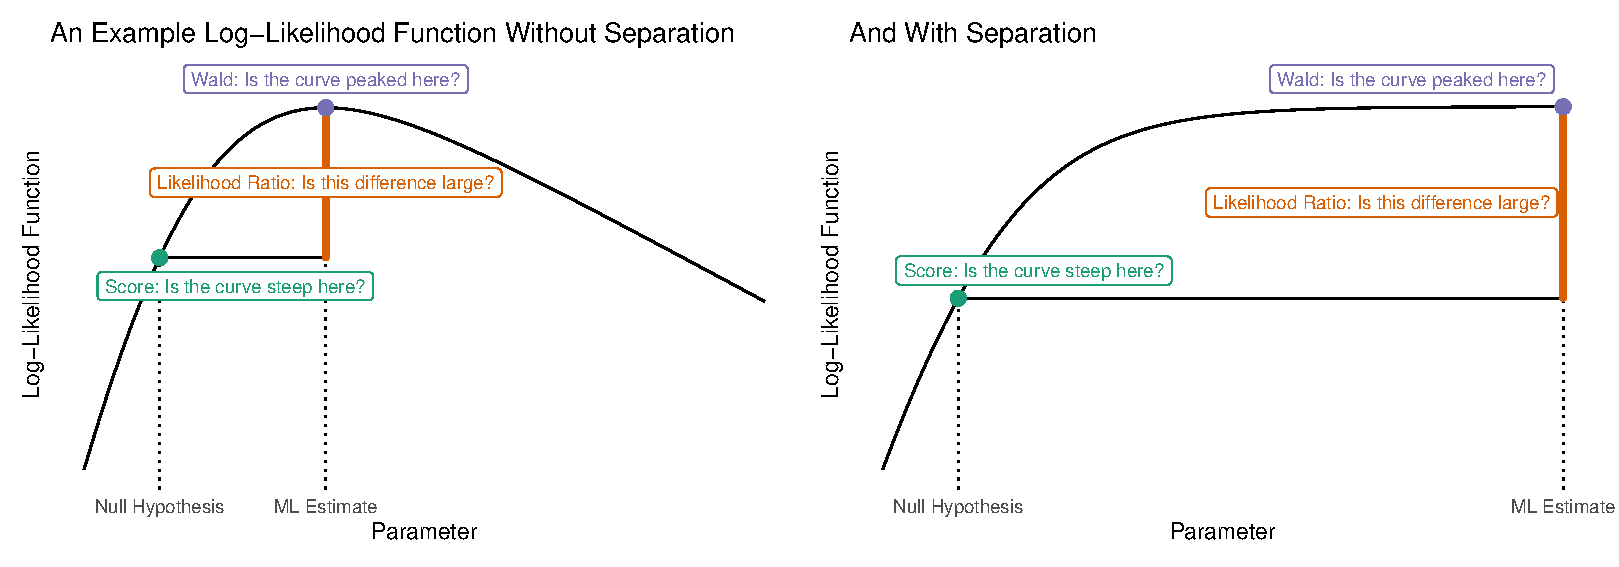
\includegraphics[width=\textwidth]{doc/fig/intuition.pdf}
\caption{A figure summarizing logic of the "holy trinity" of hypothesis tests. The Wald test relies on the curvature around the maximum of the log-likelihood function, which breaks down under separation. But the likelihood ratio and score test rely on \textit{other} features of the log-likelihood function that are not meaningfully impacted by separation.}\label{fig:trinity}
\end{figure}

We can develop the intuition of the more precisely and formally. Suppose
that a binary explanatory variable \(s\) with coefficient \(\beta_s\)
perfectly predicts the outcome \(y_i\) such that when \(s_i = 1\) then
\(y_i = 1\). Then the log-likelihood function increases in \(\beta_s\).
The standard error estimate associated with each \(\beta_s\) increases
as well. But critically, the estimated standard error increases
\emph{faster} than the associated coefficient, because
\(\lim_{\beta_s \to \infty} \left[ \left( - \dfrac{\partial^2 \ell(\beta_s | y)}{\partial^2 \beta_s} \right)^{-\frac{1}{2}} - \beta_s \right] = \infty\).
Thus, under separation, the estimated standard error will be much larger
than the coefficient for the separating variable for any algorithm that
obtains a sufficiently large coefficient. This implies two conclusions.
First, so long as the researcher uses a sufficiently precise algorithm,
\emph{the Wald test will never reject the null hypothesis}, regardless
of the data set. Second, if the Wald test can never reject the null
hypothesis for any data set with separation, then the power of the test
is strictly bounded by the chance of separation. In particular,
\emph{the power of the test cannot exceed
\(1 - Pr(\text{separation})\)}. If the data set features separation in
nearly 100\% of repeated samples, then the Wald test will have power
near 0\%.

As a final illustration, suppose an absurd example in which a binary
treatment perfectly predicts 500 successes and 500 failures (i.e.,
\(y = x\) always). Of course, this data set is \emph{extremely} unlikely
under the null hypothesis that the coefficient for the treatment
indicator equals zero. The exact \(p\)-value for the null hypothesis
that successes and failures are equally likely under both treatment and
control equals
\(2 \times \left( \frac{1}{2} \right)^{500} \times \left( \frac{1}{2} \right)^{500} = \frac{2}{2^{1000}} \approx \frac{2}{10^{301}}\).
(For comparison, there are about \(10^{80}\) atoms in the known
universe.) Yet, the default \texttt{glm()} routine in R calculates a
Wald \(p\)-value of 0.998 with the default precision (and 1.000 with the
maximum precision). When dealing with separation, the Wald test breaks
down; researchers cannot use the Wald test to obtain reasonable
\(p\)-values for the coefficient of a separating variable.

\hypertarget{likelihood-ratio-test}{%
\subsection{Likelihood Ratio Test}\label{likelihood-ratio-test}}

The likelihood ratio test resolves the problem of the flat
log-likelihood by comparing the maximum log-likelihood of two models: an
``unrestricted'' model \(ML\) that imposes no bounds on the estimates
and a ``restricted'' model \(ML_0\) that constrains the estimates to the
region suggested by the null hypothesis. If the data set is much more
likely under the unrestricted estimate than under the restricted
estimate, then the researcher can reject the null hypothesis. @Wilks1938
advises us how to compare the unrestricted log-likelihood
\(\ell(\hat{\beta}^{ML} | y)\) to the restricted log-likelihood
\(\ell(\hat{\beta}^{ML_0} | y)\):
\(D = 2 \times \left[ \ell(\hat{\beta}^{ML} | y) - \ell(\hat{\beta}^{ML_0} | y) \right]\)
approximately follows a \(\chi^2\) distribution with degrees of freedom
equal to the number of constrained dimensions (Casella and Berger 2003,
pp.~488-492, Greene 2012, pp.~526-527).

Figure \ref{fig:trinity} shows the intuition of the likelihood ratio
test. The gap between the unrestricted and restricted maximum summarizes
the evidence against the null hypothesis. Importantly, the logic does
not break down under separation. Unlike the Wald test, the likelihood
ratio test \emph{can} reject the null hypothesis under separation.

\hypertarget{score-test}{%
\subsection{Score Test}\label{score-test}}

The score test resolves the problem of the flat log-likelihood by
evaluating the gradient of the log-likelihood function at the null
hypothesis. If the log-likelihood function is increasing rapidly at the
null hypothesis, this casts doubt on the null hypothesis. The score test
uses the score function
\(S(\beta) = \dfrac{\partial \ell(\beta | y)}{\partial \beta}\) and the
Fisher information
\(I(\beta) = -E_\beta \left( \dfrac{\partial^2 \ell(\beta | y)}{\partial^2 \beta} \right)\).
When evaluated at the null hypothesis, the score function quantifies the
slope and the Fisher information quantifies the variance of that slope
in repeated samples. If the score at the null hypothesis is large, then
the researcher can reject the null hypothesis. @Rao1948 advises us how
to compare the score to its standard error:
\(Z_s = \frac{S(\beta^0_s)}{\sqrt{I(\beta^0_s)}}\) follows a standard
normal distribution (Casella and Berger 2003, pp.~494-495, Greene 2012,
pp.~529-530).

Figure \ref{fig:trinity} shows the intuition of the score test. The
slope of the log-likelihood function under the null hypothesis
summarizes the evidence against the null hypothesis. As with the
likelihood ratio test, the logic works even under separation, and the
score test \emph{can} reject the null hypothesis under separation.

Table \ref{tab:trinity} summarizes the three tests. Most importantly,
the likelihood ratio and score tests rely on features of the
log-likelihood function that are not meaningfully affected by a
monotonic log-likelihood function. The Wald test, on the other hand,
cannot provide a reasonable test under separation.

\begin{table}[h]
\scriptsize
\begin{tabular}{{p{0.12\textwidth}p{0.3\textwidth}p{0.4\textwidth}}}
Test & Feature                                                      & Statistic and Distribution      \\
\hline                                                                                  
Wald & Curvature of the log-likelihood function around the maximum. & $Z_w = \dfrac{\hat{\beta}_i^{ML}}{\widehat{\text{SE}}(\hat{\beta}_i^{ML})}$ follows a standard normal distribution.\\
 Likelihood Ratio    &   Relative log-likelihoods of the unrestricted and restricted models. &  $D = 2 \times \left[ \ell(\hat{\beta}^{ML} | y) - \ell(\hat{\beta}^{ML_0} | y) \right]$ follows a $\chi^2$ distribution with degrees of freedom equal to the number of constrained dimensions. \\
 Score    &   Slope of the log-likelihood function \textit{at the null hypothesis}.                                                            &   $Z_s = \frac{S(\beta^0_s)}{\sqrt{I(\beta^0_s)}}$ follows a standard normal distribution.
\end{tabular}\caption{A table summarizing the "holy trinity" of hypothesis tests.}\label{tab:trinity}
\end{table}

\hypertarget{simulations}{%
\section{Simulations}\label{simulations}}

To evaluate the performance of the three tests under separation, I use a
diverse collection of data-generating processes (DGPs). Each DGP
features separation in more than 10\% of repeated samples. Importantly,
I cannot focus on data sets \emph{with separation} because separation is
a feature of a particular sample. Instead, I focus on DGPs that
\emph{sometimes} feature separation (e.g., in 15\% of repeated samples,
in 50\% of repeated samples, etc.).

To create the collection of DGPs, I imagine the logistic regression
model
\(\Pr(y = 1) = \text{logit}^{-1}(\beta_{\text{cons}} + \beta_s s + \beta_{z_1} z_1 + ... + \beta_{z_k} z_k)\)
and a researcher testing the null hypothesis that the binary explanatory
variable \(s\) (that might produce separation) has no effect on a binary
outcome variable \(y\) (i.e., that \(\beta_s = 0\)). I vary the total
number of observations, the frequency that \(s = 1\), the value of
\(\beta_{\text{cons}}\), and the number of control variables
(\(k\)).\footnote{Each control variable \(z_i\) is simulated from a
  normal distribution with a standard deviation of 0.5. The coefficient
  for each control variable \(\beta_{z_i}\) is set to one.} For each
DGP, I use Monte Carlo simulation to compute the power function for each
of the three tests.

\hypertarget{a-close-look-at-a-single-dgp}{%
\subsection{A Close Look at a Single
DGP}\label{a-close-look-at-a-single-dgp}}

Following the structure discussed above, I first examine a single DGP.
There are 50 total observations, \(s = 1\) for five of the observations
and \(s = 0\) for the other 45 observations, the intercept
\(\beta_{cons}\) is zero, and there are two control variables. Table
\ref{tab:single-dgp-pwr} shows the power function for each of the three
tests and the percent of the data sets that featured separation for the
parameter combination and the value of \(\beta_s\). For this particular
DGP, separation is relatively rare when \(\beta_s\)---the coefficient
for the potentially separating variable---is near zero. But for
\(\beta_s = \pm 2\), about 50\% of the data sets feature separation. And
for \(\beta_s\) larger/smaller than \(\pm 4\), more than 90\% of the
data sets feature separation.

\renewcommand{\captiontext}{}
\renewcommand{\notetext}{This table shows the power for the Wald, likelihood ratio, and score tests for a DGP that often features separation.}
\begin{table}[!h]
\caption{\label{tab:single-dgp-pwr}}
\centering
\fontsize{8}{9}\selectfont
\begin{threeparttable}

\begin{tabular}{>{}cccccccc}
\toprule
$\beta_s$ & Ideal Power & Chance of Separation & ML w/ Wald & ML w/ LR & ML w/ Score & PML (Firth) w/ Wald & PML (Cauchy) w/ Wald\\
\midrule
5.00 &  & 81\% & 20\% & 100\% & 100\% & 100\% & 100\%\\

4.00 &  & 58\% & 43\% & 100\% & 100\% & 99\% & 99\%\\

3.00 &  & 25\% & 72\% & 98\% & 98\% & 95\% & 96\%\\

2.00 &  & 3\% & 71\% & 76\% & 77\% & 68\% & 70\%\\

1.00 &  & 0\% & 26\% & 28\% & 30\% & 22\% & 22\%\\

0.75 &  & 0\% & 16\% & 17\% & 19\% & 13\% & 14\%\\

0.50 &  & 1\% & 10\% & 11\% & 12\% & 8\% & 8\%\\

0.40 &  & 1\% & 7\% & 9\% & 9\% & 5\% & 5\%\\

0.30 &  & 1\% & 6\% & 8\% & 8\% & 5\% & 5\%\\

0.20 &  & 2\% & 5\% & 7\% & 6\% & 4\% & 4\%\\

0.10 & \multirow{-11}{*}{\centering\arraybackslash As high as possible.} & 2\% & 3\% & 7\% & 6\% & 3\% & 3\%\\
\addlinespace
0.00 & 5\% & 3\% & 2\% & 6\% & 5\% & 2\% & 2\%\\
\addlinespace
-0.10 &  & 4\% & 2\% & 6\% & 4\% & 2\% & 2\%\\

-0.20 &  & 5\% & 2\% & 10\% & 6\% & 2\% & 2\%\\

-0.30 &  & 6\% & 1\% & 9\% & 6\% & 1\% & 1\%\\

-0.40 &  & 8\% & 1\% & 9\% & 5\% & 1\% & 1\%\\

-0.50 &  & 10\% & 1\% & 12\% & 6\% & 1\% & 1\%\\

-0.75 &  & 16\% & 1\% & 18\% & 10\% & 1\% & 2\%\\

-1.00 &  & 23\% & 0\% & 25\% & 15\% & 0\% & 2\%\\

-2.00 &  & 56\% & 0\% & 54\% & 30\% & 1\% & 5\%\\

-3.00 &  & 80\% & 0\% & 76\% & 42\% & 1\% & 6\%\\

-4.00 &  & 92\% & 0\% & 86\% & 48\% & 1\% & 6\%\\

-5.00 & \multirow{-11}{*}{\centering\arraybackslash As high as possible.} & 97\% & 0\% & 90\% & 51\% & 1\% & 6\%\\
\bottomrule
\end{tabular}   
\begin{tablenotes}[para]
This table shows the power for the Wald, likelihood ratio, and score tests for a DGP that often features separation.
\end{tablenotes}
\end{threeparttable}
\end{table}

This DGP clearly demonstrates the poor performance of the Wald test.
Even though the data sets with separation should allow the researcher to
reject the null hypothesis, at least occasionally, the power of the Wald
test is near 0\% even for very large effects. This happens because the
Wald test cannot reject the null hypothesis under separation. When
separation happen often, the power \emph{must} be low. The likelihood
ratio and score tests, on the other hand, perform as expected. For both
alternatives, the power of the test when \(\beta_s = 0\) is about 5\%,
as designed, and the power approaches 100\% relatively quickly as
\(\beta_s\) moves away from zero.

\hypertarget{a-broad-look-at-many-dgps}{%
\subsection{A Broad Look at Many DGPs}\label{a-broad-look-at-many-dgps}}

Table \ref{tab:many-dgps-pars} shows the broad collection of parameters
I used in the simulations. All combinations of the values below yield
150 unique combinations. I exclude combinations in which the frequency
that \(s = 1\) exceeded the number of observations, which leaves 110
combinations. For each of these 110 combinations, I use Monte Carlo
simulations to estimate the probability that each method rejects the
null hypothesis as the coefficient \(\beta_s\) varies from -10 to 10
(across the particular values shown in Table \ref{tab:single-dgp-pwr}).
I also exclude any scenario in which the parameter and the coefficient
\(\beta_s\) would sometimes produce data sets with no variation in the
outcome variable. As such, one might consider this a diverse collection
of DGPs that sometimes generate separation but almost always have
variation in the outcome.

\renewcommand{\captiontext}{}
\renewcommand{\notetext}{}
\begin{table}[!h]
\caption{\label{tab:many-dgps-pars}}
\centering
\fontsize{10}{12}\selectfont
\begin{threeparttable}
\begin{tabular}{lc}
\toprule
Parameter & Value        \\
\midrule
Total Number of Observations & 50, 250, 500 \\
Frequency that $s = 1$    &   5, 25, 50, 100, 250 \\
The Value of the Intercept $\beta_{\text{cons}}$ & -8, -5, -2.5, -1, 0 \\
The Number of Control Variables $k$ & 2, 6 \\
\bottomrule
\end{tabular}\begin{tablenotes}[para]

\end{tablenotes}
\end{threeparttable}
\end{table}

Figure \ref{fig:many-sims} shows the statistical power of each of the
three tests as the chance of separation varies across the many DGPs.
Most starkly, the power of the Wald test is bounded above by
\(1 - Pr(\text{separation})\), and many scenarios achieve the boundary.
Intuitively, as the chance of separation increases, the power of the
test should increase as well, because separation is evidence of a large
coefficient. But because a large coefficient makes separation more
likely, a large coefficient \emph{decreases} the power of the Wald test.
The likelihood ratio and score test, on the other hand, behave as
expected.

\begin{figure}[h]
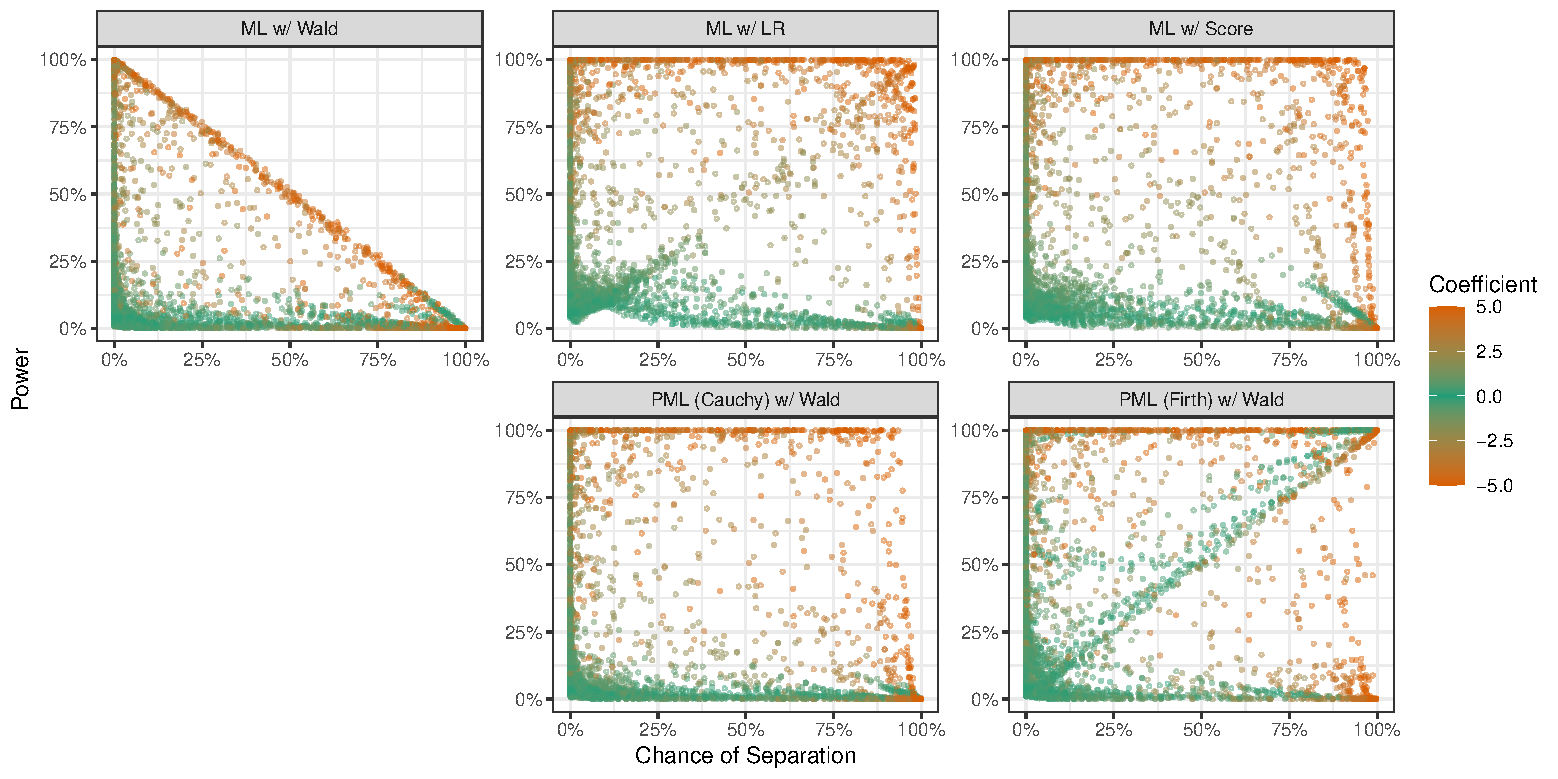
\includegraphics[width=\textwidth]{doc/fig/many-sims.pdf}
\caption{The power of tests across a range of scenarios as the chance of separation varies.}\label{fig:many-sims}
\end{figure}

Figure \ref{fig:power-funs} plots the power function for each of the 110
DGPs in the diverse collection.\footnote{I exclude parameter
  combinations that might not produce variation in the outcome variable,
  so I do not compute the power function across the entire range of the
  coefficient for every power function. For 47 of the 110 DGPs, I
  exclude a portion of the range. For 63 of the 110, I compute the power
  function across the entire range from -10 to 10.} The fine lines show
the power function for each DGP and the color of the points indicates
the chance of separation at that point. The heavy, solid lines show the
average of the collection of power functions. The heavy, dashed lines
show the power functions for the other two tests, for comparison.

First, the power functions for the Wald tests show its poor properties.
For most of the power functions, as the true coefficient grows larger in
magnitude from about three, the test becomes less powerful. This occurs
because separation becomes more likely and the test cannot reject the
null hypothesis when separation occurs. Second, the likelihood ratio and
score test behave reasonably well. Most importantly, the size of the
likelihood ratio and score tests is about 5\% when the coefficient
equals zero and grows as the coefficient moves away from zero. The
likelihood ratio test is slightly preferred, at least of this collection
of DGPs, because it is slightly more powerful when the coefficient does
not equal zero, especially for large, negative coefficients.\footnote{This
  asymmetry occurs because I only consider negative intercepts.}

\begin{figure}[!h]
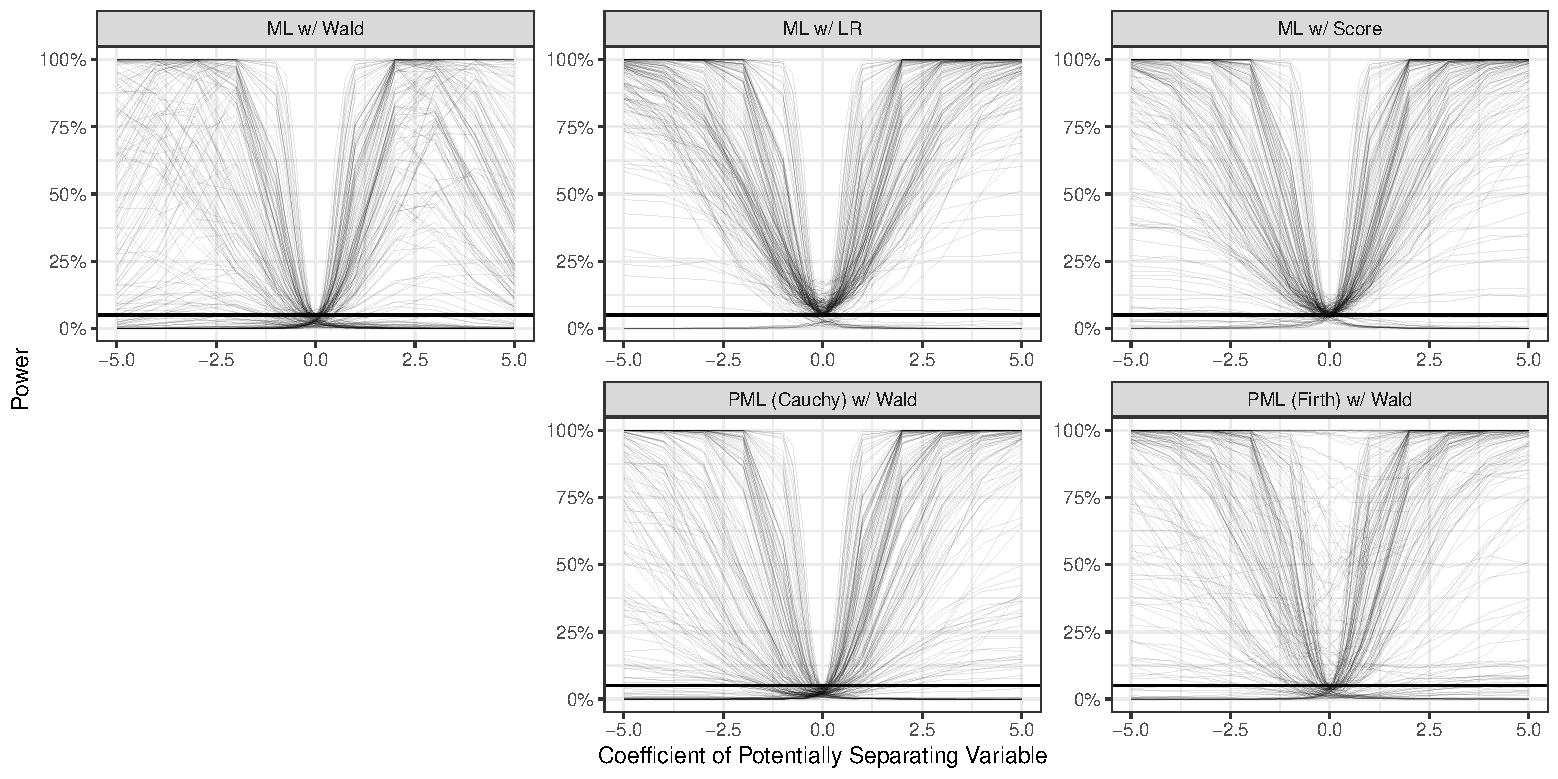
\includegraphics[scale = 0.7]{doc/fig/power-funs.pdf}
\caption{The power functions for the Wald, likelihood ratio, and score tests for a diverse collection of data-generating processes that sometimes generate separation.}\label{fig:power-funs}
\end{figure}

\hypertarget{practical-advice}{%
\section{Practical Advice}\label{practical-advice}}

Given the arguments above, how should researchers proceed when facing
separation? I offer the following {[}ADD NUMBER HERE{]} pieces of
advice, which incorporate my advice with the larger literature.

\begin{enumerate}
\def\labelenumi{\arabic{enumi}.}
\tightlist
\item
  \emph{Identify separation.} Software varies in how and whether it
  detects and reports the presence of separation. Become familiar with
  your preferred software.\footnote{As of this writing, the
    \texttt{glm()} function in R \emph{sometimes} reports a warning that
    ``fitted probabilities numerically 0 or 1 occurred.'' The researcher
    must detect separation by noticing the unusually large coefficient
    estimate and standard error. Stata's \texttt{logit} and
    \texttt{probit} commands print a ``note'' that describes the
    separation. It then drops the problematic variable and the
    observations it perfectly predicts.}
\item
  \emph{Do not drop the separating variable.} If a variable creates
  separation, then researchers might be tempted to drop the offending
  variable. This is poor practice. See Zorn (2005) for more details.
\item
  \emph{Test the hypothesis about the effect of the separating
  variable}. While the point estimates might be implausible and the Wald
  \(p\)-values nonsensical, researchers can still use a likelihood ratio
  and/or score test to obtain a useful \(p\)-value and test the null
  hypothesis that the coefficient for the separating variable equals
  zero. If the coefficient of the separating variable is not of
  substantive interest (i.e., the researcher does not have a specific
  hypothesis about its value; the researcher includes the separating
  variable only as a control), then there is no need to perform this
  hypothesis test. The researcher can report this test in the text of
  the paper and/or in a regression table, carefully distinguishing the
  likelihood ratio and/or score tests from the Wald test readers expect.
\item
  \emph{Estimate the coefficients and uncertainty using penalized
  maximum likelihood or Bayesian estimation}. Firth (1993) and Gelman et
  al.~(2008) offer reasonable default penalties or prior distributions
  that might work well for a given substantive application. However,
  Rainey (2016) shows that the inferences can meaningfully depend on the
  chosen penalty or prior. With this sensitivity in mind, the researcher
  should choose the penalty or prior \emph{carefully} and/or check the
  robustness of their conclusions to alternative prior
  specifications.\footnote{The simulations above suggest that
    researchers should be especially skeptical of the \(p\)-values from
    the Firth penalty. The simulations show that the Firth \(p\)-values
    can reject the null hypothesis incorrectly at well above the nominal
    rate for a variable that often creates separation.}
\item
  \emph{Compute substantively meaningful quantities of interest and
  uncertainty}. Researchers using penalized maximum likelihood can use
  the informal posterior simulation procedure suggested by King, Tomz,
  and Wittenberg (2001) (see also Gelman and Hill 2006; Bell and Miller
  YYYY for an example.) to compute point estimates and confidence
  intervals for the quantities of interest. Researchers using full
  posterior simulation can transform the simulations of the model
  coefficients to obtain posterior simulations of the quantities of
  interest.
\end{enumerate}

\hypertarget{re-analysis-of-barrilleaux-and-rainey-2014}{%
\section{Re-Analysis of Barrilleaux and Rainey
(2014)}\label{re-analysis-of-barrilleaux-and-rainey-2014}}

To illustrate the power and simplicity of frequentist hypothesis testing
under separation, I reanalyze data from @BarrilleauxRainey2014, who
examine U.S. state governors decisions to support or oppose the Medicaid
expansion under the 2010 Affordable Care Act. But because all Democratic
governors supported the expansion, separation occurs---being a
Democratic governor perfectly predicts support for Medicaid expansion.

I focus on their first hypothesis: \emph{Republican governors are more
likely to oppose the Medicaid expansion funds than Democratic
governors.} Barrilleaux and Rainey adopt a fully Bayesian approach,
modeling the probability that a state's governor opposes the Medicaid
expansion as a function of the governor's partisanship and several other
covariates. Here, I re-estimate their logistic regression model and
compute Wald, likelihood ratio, and score \(p\)-values. Table
\ref{tab:br-p} presents the estimates and \(p\)-values for the
coefficient of the binary Democratic governor variable. While the Wald
\(p\)-value is near 1.00, the likelihood ratio and score tests produce
more plausible \(p\)-values of 0.003 and 0.009, respectively.\footnote{For
  comparison, the Wald tests for the Jeffreys and Cauchy penalized
  maximum likelihood estimators produce \(p\)-values of 0.060 and 0.038,
  respectively.}

\renewcommand{\captiontext}{}
\renewcommand{\notetext}{The $p$-values from several procedures that researchers might use when dealing with separation in logistic regression models. The Wald test for maximum likelihood estimates relies on unreasonable standard errors that depend heavily on the precision of the algorithm and, as a consequence, produces unrealistic $p$-values. However, the likelihood ratio and score tests produce reasonable $p$-values.}
\begin{table}[!h]
\caption{\label{tab:br-p}}
\centering
\fontsize{10}{12}\selectfont
\begin{threeparttable}

\begin{tabular}{lcccc}
\toprule
\textbf{Estimator} & \textbf{Coef. Est.} & \textbf{SE Est.} & \textbf{Wald \textit{p}-Value} & \textbf{LR \textit{p}-Value}\\
\midrule
ML with Default Precision & -20.35 & 3,224 & 0.99 & 0.00\\
ML with Maximum Precision & -35.22 & 15 million & 1.00 & 0.00\\
PML with Jeffreys Penalty & -2.68 & 1.42 & 0.06 & \\
PML with Cauchy Penalty & -3.38 & 1.63 & 0.04 & \\
\bottomrule
\end{tabular}
\begin{tablenotes}[para]
The $p$-values from several procedures that researchers might use when dealing with separation in logistic regression models. The Wald test for maximum likelihood estimates relies on unreasonable standard errors that depend heavily on the precision of the algorithm and, as a consequence, produces unrealistic $p$-values. However, the likelihood ratio and score tests produce reasonable $p$-values.
\end{tablenotes}
\end{threeparttable}
\end{table}

% Table generated by Excel2LaTeX from sheet 'Sheet1'
\begin{table}[htbp]
  \centering
  \caption{Add caption}
    \begin{tabular}{lrrrrrrrrrrrr}
    \textcolor[rgb]{ .2,  .2,  .2}{} & \multicolumn{1}{l}{\textcolor[rgb]{ .2,  .2,  .2}{ML w/ Default Precision}} & \multicolumn{1}{l}{\textcolor[rgb]{ .2,  .2,  .2}{ML w/ Maximum Precision}} & \multicolumn{1}{l}{\textcolor[rgb]{ .2,  .2,  .2}{PML w/ Firth's Penalty}} & \multicolumn{1}{l}{\textcolor[rgb]{ .2,  .2,  .2}{PML w/ Cauchy Penalty}} &       &       &       &       &       &       &       &  \\
    \textcolor[rgb]{ .2,  .2,  .2}{Est.} & \multicolumn{1}{l}{\textcolor[rgb]{ .2,  .2,  .2}{S.E.}} & \multicolumn{1}{l}{\textcolor[rgb]{ .2,  .2,  .2}{p}} & \multicolumn{1}{l}{\textcolor[rgb]{ .2,  .2,  .2}{Est.}} & \multicolumn{1}{l}{\textcolor[rgb]{ .2,  .2,  .2}{S.E.}} & \multicolumn{1}{l}{\textcolor[rgb]{ .2,  .2,  .2}{p}} & \multicolumn{1}{l}{\textcolor[rgb]{ .2,  .2,  .2}{Est.}} & \multicolumn{1}{l}{\textcolor[rgb]{ .2,  .2,  .2}{S.E.}} & \multicolumn{1}{l}{\textcolor[rgb]{ .2,  .2,  .2}{p}} & \multicolumn{1}{l}{\textcolor[rgb]{ .2,  .2,  .2}{Est.}} & \multicolumn{1}{l}{\textcolor[rgb]{ .2,  .2,  .2}{S.E.}} & \multicolumn{1}{l}{\textcolor[rgb]{ .2,  .2,  .2}{p}} &  \\
    \textcolor[rgb]{ .2,  .2,  .2}{(Intercept)} & \textcolor[rgb]{ .2,  .2,  .2}{-8.855} & \textcolor[rgb]{ .2,  .2,  .2}{1289.76} & \textcolor[rgb]{ .2,  .2,  .2}{0.995} & \textcolor[rgb]{ .2,  .2,  .2}{-14.865} & \textcolor[rgb]{ .2,  .2,  .2}{6002399} & \textcolor[rgb]{ .2,  .2,  .2}{1} & \textcolor[rgb]{ .2,  .2,  .2}{-1.496} & \textcolor[rgb]{ .2,  .2,  .2}{0.604} & \textcolor[rgb]{ .2,  .2,  .2}{0.013} & \textcolor[rgb]{ .2,  .2,  .2}{-1.913} & \textcolor[rgb]{ .2,  .2,  .2}{0.758} & \textcolor[rgb]{ .2,  .2,  .2}{0.012} \\
    \textcolor[rgb]{ .2,  .2,  .2}{dem\_governor} & \textcolor[rgb]{ .2,  .2,  .2}{-20.349} & \textcolor[rgb]{ .2,  .2,  .2}{3224.4} & \textcolor[rgb]{ .2,  .2,  .2}{0.995} & \textcolor[rgb]{ .2,  .2,  .2}{-35.375} & \textcolor[rgb]{ .2,  .2,  .2}{1.5E+07} & \textcolor[rgb]{ .2,  .2,  .2}{1} & \textcolor[rgb]{ .2,  .2,  .2}{-2.677} & \textcolor[rgb]{ .2,  .2,  .2}{1.421} & \textcolor[rgb]{ .2,  .2,  .2}{0.06} & \textcolor[rgb]{ .2,  .2,  .2}{-3.379} & \textcolor[rgb]{ .2,  .2,  .2}{1.631} & \textcolor[rgb]{ .2,  .2,  .2}{0.038} \\
    \textcolor[rgb]{ .2,  .2,  .2}{percent\_favorable\_aca} & \textcolor[rgb]{ .2,  .2,  .2}{0.128} & \textcolor[rgb]{ .2,  .2,  .2}{1.549} & \textcolor[rgb]{ .2,  .2,  .2}{0.934} & \textcolor[rgb]{ .2,  .2,  .2}{0.128} & \textcolor[rgb]{ .2,  .2,  .2}{1.549} & \textcolor[rgb]{ .2,  .2,  .2}{0.934} & \textcolor[rgb]{ .2,  .2,  .2}{-0.138} & \textcolor[rgb]{ .2,  .2,  .2}{1.313} & \textcolor[rgb]{ .2,  .2,  .2}{0.916} & \textcolor[rgb]{ .2,  .2,  .2}{-0.208} & \textcolor[rgb]{ .2,  .2,  .2}{1.035} & \textcolor[rgb]{ .2,  .2,  .2}{0.84} \\
    \textcolor[rgb]{ .2,  .2,  .2}{gop\_leg} & \textcolor[rgb]{ .2,  .2,  .2}{2.429} & \textcolor[rgb]{ .2,  .2,  .2}{1.48} & \textcolor[rgb]{ .2,  .2,  .2}{0.101} & \textcolor[rgb]{ .2,  .2,  .2}{2.429} & \textcolor[rgb]{ .2,  .2,  .2}{1.48} & \textcolor[rgb]{ .2,  .2,  .2}{0.101} & \textcolor[rgb]{ .2,  .2,  .2}{1.618} & \textcolor[rgb]{ .2,  .2,  .2}{1.174} & \textcolor[rgb]{ .2,  .2,  .2}{0.168} & \textcolor[rgb]{ .2,  .2,  .2}{1.696} & \textcolor[rgb]{ .2,  .2,  .2}{1.061} & \textcolor[rgb]{ .2,  .2,  .2}{0.11} \\
    \textcolor[rgb]{ .2,  .2,  .2}{percent\_uninsured} & \textcolor[rgb]{ .2,  .2,  .2}{0.923} & \textcolor[rgb]{ .2,  .2,  .2}{2.234} & \textcolor[rgb]{ .2,  .2,  .2}{0.68} & \textcolor[rgb]{ .2,  .2,  .2}{0.923} & \textcolor[rgb]{ .2,  .2,  .2}{2.234} & \textcolor[rgb]{ .2,  .2,  .2}{0.68} & \textcolor[rgb]{ .2,  .2,  .2}{0.18} & \textcolor[rgb]{ .2,  .2,  .2}{1.127} & \textcolor[rgb]{ .2,  .2,  .2}{0.873} & \textcolor[rgb]{ .2,  .2,  .2}{0.6} & \textcolor[rgb]{ .2,  .2,  .2}{1.078} & \textcolor[rgb]{ .2,  .2,  .2}{0.578} \\
    \textcolor[rgb]{ .2,  .2,  .2}{bal2012} & \textcolor[rgb]{ .2,  .2,  .2}{-0.054} & \textcolor[rgb]{ .2,  .2,  .2}{0.854} & \textcolor[rgb]{ .2,  .2,  .2}{0.95} & \textcolor[rgb]{ .2,  .2,  .2}{-0.054} & \textcolor[rgb]{ .2,  .2,  .2}{0.854} & \textcolor[rgb]{ .2,  .2,  .2}{0.95} & \textcolor[rgb]{ .2,  .2,  .2}{-0.123} & \textcolor[rgb]{ .2,  .2,  .2}{0.725} & \textcolor[rgb]{ .2,  .2,  .2}{0.865} & \textcolor[rgb]{ .2,  .2,  .2}{0.155} & \textcolor[rgb]{ .2,  .2,  .2}{0.751} & \textcolor[rgb]{ .2,  .2,  .2}{0.837} \\
    \textcolor[rgb]{ .2,  .2,  .2}{multiplier} & \textcolor[rgb]{ .2,  .2,  .2}{-0.355} & \textcolor[rgb]{ .2,  .2,  .2}{1.193} & \textcolor[rgb]{ .2,  .2,  .2}{0.766} & \textcolor[rgb]{ .2,  .2,  .2}{-0.355} & \textcolor[rgb]{ .2,  .2,  .2}{1.193} & \textcolor[rgb]{ .2,  .2,  .2}{0.766} & \textcolor[rgb]{ .2,  .2,  .2}{-0.326} & \textcolor[rgb]{ .2,  .2,  .2}{1.018} & \textcolor[rgb]{ .2,  .2,  .2}{0.748} & \textcolor[rgb]{ .2,  .2,  .2}{-0.162} & \textcolor[rgb]{ .2,  .2,  .2}{0.877} & \textcolor[rgb]{ .2,  .2,  .2}{0.853} \\
    \textcolor[rgb]{ .2,  .2,  .2}{percent\_nonwhite} & \textcolor[rgb]{ .2,  .2,  .2}{1.434} & \textcolor[rgb]{ .2,  .2,  .2}{2.616} & \textcolor[rgb]{ .2,  .2,  .2}{0.584} & \textcolor[rgb]{ .2,  .2,  .2}{1.434} & \textcolor[rgb]{ .2,  .2,  .2}{2.616} & \textcolor[rgb]{ .2,  .2,  .2}{0.584} & \textcolor[rgb]{ .2,  .2,  .2}{1.562} & \textcolor[rgb]{ .2,  .2,  .2}{1.208} & \textcolor[rgb]{ .2,  .2,  .2}{0.196} & \textcolor[rgb]{ .2,  .2,  .2}{0.934} & \textcolor[rgb]{ .2,  .2,  .2}{1.245} & \textcolor[rgb]{ .2,  .2,  .2}{0.453} \\
    \textcolor[rgb]{ .2,  .2,  .2}{percent\_metro} & \textcolor[rgb]{ .2,  .2,  .2}{-2.759} & \textcolor[rgb]{ .2,  .2,  .2}{1.687} & \textcolor[rgb]{ .2,  .2,  .2}{0.102} & \textcolor[rgb]{ .2,  .2,  .2}{-2.759} & \textcolor[rgb]{ .2,  .2,  .2}{1.687} & \textcolor[rgb]{ .2,  .2,  .2}{0.102} & \textcolor[rgb]{ .2,  .2,  .2}{-1.82} & \textcolor[rgb]{ .2,  .2,  .2}{1.188} & \textcolor[rgb]{ .2,  .2,  .2}{0.126} & \textcolor[rgb]{ .2,  .2,  .2}{-1.46} & \textcolor[rgb]{ .2,  .2,  .2}{1.044} & \textcolor[rgb]{ .2,  .2,  .2}{0.162} \\
    \end{tabular}%
  \label{tab:addlabel}%
\end{table}%


\hypertarget{conclusion}{%
\section{Conclusion}\label{conclusion}}

Separation commonly occurs in political science. When this happens, I
show that the usual Wald \(p\)-values are highly misleading. But
researchers cannot always use prior information to address a monotonic
likelihood function. Even without a suitable prior or penalty, I show
that the standard likelihood ratio and score tests behave in the usual
way. As such, researchers can use the likelihood ratio and score tests
to produce meaningful \(p\)-values under separation \emph{without the
use of prior information}.

\newpage

\hypertarget{references}{%
\section{References}\label{references}}

\setlength{\parindent}{-0.2in}
\setlength{\leftskip}{0.2in}
\setlength{\parskip}{8pt}

\noindent

\end{document}
